
% ---------------------------------------------------------------------------------------------------------------
\chapter{Introduction}
\label{ch:intro}
% ---------------------------------------------------------------------------------------------------------------
Curiosity is the driving force behind the development of human civilisation. Over centuries, scientists have discovered new methods for understanding Nature and the fundamental mechanisms governing the Universe, using continually improving research methods and technology to peer ever deeper into the heart of matter.

After the initial discovery of atoms, their underlying structure was soon revealed to be that of a positively charged core surrounded by a cloud of orbiting electrons. The atomic nucleus was subsequently decomposed into protons and neutrons, which themselves were found to consist of three tiny quarks. Studying these minuscule building blocks of visible matter has made it possible to understand more about the intricate complexities of the Universe, and the mechanisms that guide its behaviour and evolution.

Discoveries of this magnitude would not have been possible without the technologies developed to carry out such experiments. On one hand, the energy of the experimental devices has been increasing continually, allowing smaller and smaller distance scales to be probed. On the other hand, the devices used to observe and measure the phenomena created in these experiments have had to be designed with improved precision, speed and durability. 

Keeping these factors in mind, the goal of this work was to find ``the perfect material''. Diamond proved to be a worthy contender, offering both outstanding electrical and mechanical properties which make it the material of choice for a number of applications in experimental physics. However, much remains to be learned about its behaviour, and this thesis adds a small piece to the shimmering mosaic of diamond research efforts.

The first chapter introduces some of the leading particle physics research institutes, and describes how their research is carried out. The second chapter discusses the properties of diamond detectors used in high energy particle physics experiments. A diamond sensor irradiation study is presented in chapter 3. The conclusions of this study, which define the constraints for the two diamond detector applications, are presented in the final two chapters.




%The aim of the thesis is to present and discuss applications of diamond based particle detectors. 
%
%The introductory chapter paints a picture of the current state of particle physics research. It presents some of the research institutes that are active in this field, pushing the boundaries of human knowledge further. It explains their goals and the means with which they are achieving them. Next section describes particle detectors in a broad sense -- their history and the types existing now. One type in particular -- a diamond detector -- is then described more in detail.
%
%The second chapter discusses the properties of diamond detectors. First it explains the detector chain into individual parts and describes them in detail -- sensors, amplifiers, digitisers and signal processing units. Second, it contains information about energy resolution in diamond, the analog and digital noise contribution, etc. Third, it presents the principles of signal formation, starting with the famous Shockley-Ramo theorem and building from there. It uses the theorem to show that different types of radiation induce different electrical signal shapes.
%
%The base laid down in the second chapter is complemented in the third where the measurements are presented and the results discussed. The chapter focuses on charge measurement stability with respect to irradiation damage.
%
%Building on the understanding of the behaviour of the diamond, two applications were developed. The fourth chapter describes the Diamond Beam Monitor, a detector that makes use of the diamond's charge measurement capabilities and its high radiation hardness. This detector has been installed in one of the largest particle physics experiments in the world and is currently taking data. Here, its development process is presented: the quality control procedures during assembly and installation, its performance in the test environment and some recent experimental data.
%
%The final and most important chapter describes the real-time application for particle identification. Here the shape of the current signal of the diamond sensor is used to discriminate different types of radiation in real time. The chapter includes the description of the device's logic and algorithms, experimental results and applications in neutron monitoring.

 




% ---------------------------------------------------------------------------------------------------------------
\clearpage
\section{Fundamental research}
\label{sec:fundphy}
% ---------------------------------------------------------------------------------------------------------------
The aim of fundamental research is to define scientific theories and verify them to improve our understanding of the universe. It does not in itself focus on applying this research by developing products and is not meant to create a direct return on investment. Instead, it expands the overall knowledge of the human kind - by making the results freely available to the general public.

Particle physics research peers into the smallest constituents of the universe, dissecting the atoms into quarks and electrons, catching cosmic rays and figuring out what dark matter is made of. Particle physicists want to explain the phenomena surrounding us by studying the fundamental particles and the mechanisms governing their interactions. By understanding this, we would be able to answer difficult questions; How did the universe begin? What is the invisible force (dark matter, dark energy) pushing the galaxies apart from each other? Where does mass come from? Why is there almost no antimatter in the universe? In this effort, scientists have formed several theories. One of them, the Standard Model of particles, is currently the most successful theory to describe the constituents of matter and their interactions.

\begin{description}
\item[The Standard Model]
(SM) is a physics theory developed in the 1970's~\cite{Novaes:1999yn}. It was designed to explain the current experimental results. As such, it was also able to predict new discoveries and was a driving force for the scientists to invest time and money in developing new experiments. To date, it is by far the most established and verified physics theory. It explains how the basic building blocks of matter -- \emph{fermions} -- interact with each other via mediators of interactions called \emph{bosons}.  
\begin{figure}[!t]
\centering
\includegraphics[width=0.9\textwidth]{01_introduction/pics/sm}
\caption{The Standard model \cite{Dominguez:2002395}.}
\label{fig:sm1}
\end{figure}
There are two main families of fermions - \emph{quarks} and \emph{leptons}, as shown in figure~\ref{fig:sm1}. Each group consists of six members divided into three \emph{generations}, the first being the lightest and most stable and the last the heaviest, which are the most unstable. The nature around us is made up of the stable particles -- those from the second or third generations can only be found in cosmic rays or produced artificially using particle accelerators.

Quarks have a spin of 1/2 and a charge of either +2/3 (up, charm, top)  or -1/3  (down, strange, bottom) while the leptons have a spin of 1/2  and a charge of either 1 (electron, muon, tau) or 0 (electron neutrino, muon neutrino, tau neutrino). Leptons only exist individually -- they do not cluster. Quarks, however, immediately form a cluster of either two (unstable), three (more stable) or five (unstable). Two up and one down quark make up a proton whereas two down and one up quark make up a neutron.

In addition to fermions, each particle has its corresponding antiparticle -- a particle with the same mass but the opposite charge. If an antiparticle hits a particle, they annihilate each other, producing energy in form of photons. 

Bosons are the carriers of force that mediate weak (W$^+$, W$^-$ and Z bosons), strong (gluons) and electromagnetic (photons) interactions. The weak interaction is responsible for the radioactive decay of subatomic particles, thus playing an essential role in nuclear fusion -- a process taking place in the stars. The electromagnetic interaction works at a macroscopic level -- it allows particles to interact via electric and magnetic fields. The strong interaction is effective at femtometer distances and it governs how quarks interact and bind with each other. An additional boson is the Higgs boson discovered at CERN in 2012~\cite{}. It is a representation of the Higgs mechanism, which gives rise to the mass (or lack thereof) of all the particles in the Standard Model.
\end{description}

\section{Research institutes}
This section gives a short overview of some of the institutes and collaborations carrying out fundamental physics research. These facilities were used for the research carried out for this thesis. 


\begin{description}
\item[CERN] (European Centre for Nuclear Research)~\cite{CERN:00000} is the largest particle physics laboratory in the world, straddling the Swiss-French border just outside Geneva. It was established in 1954 to bring the war-torn Europe together by means of fundamental scientific research. Today, its 22 member state countries and several observer states contribute approximately 1~billion CHF annually to fund the research and development. More than 10000 scientists, engineers, technicians, students and others from all around the globe work at CERN on many projects in research fields ranging from particle to nuclear physics. The scope is to probe the fundamental structure of the universe and to understand the mechanisms governing it. Therefore CERN's main function is to provide the infrastructure for high-energy physics experiments. These are carried out using large machines called particle accelerators. These instruments boost beams of particles to high energies before making them collide with each other or with stationary targets. The resulting collisions are recorded by particle detectors and later analysed by physicists. To carry out research on the smallest constituents of matter, their dynamics and structure, very high energies are needed. This is why the most powerful accelerators are used for fundamental research. The largest accelerators at CERN are the Proton Synchrotron~\cite{}, the Super Proton Synchrotron~\cite{Mills:133232} and the Large Hadron Collider, described in~\ref{subsec:lhc}.



\item[Atominstitut, Vienna] (ATI)~\cite{AtomInst:00000}, an institute for atomic and subatomic physics, was established in 1958 in Vienna as an inter-university institute. It houses around 200 people involved in a broad range of research fields: quantum, particle, neutron, nuclear, radiation and reactor physics, quantum optics etc. As of 2002 the ATI is part of the University of Technology in Vienna.

Its central facility is \emph{TRIGA MARK II}~\cite{Triga:00000}, a neutron reactor used for training, research and isotope production. It is one of 40 such reactors worldwide, produced by the Californian company General Atomic in the early 60's. It is capable of continuous operation at a maximum output power of 250~kW. 
The reactor core consists of 3~kg of 20~\% enriched uranium ($^{235}$U). The fuel moderator rods are mostly made up of zirconium with low percentage of hydrogen and uranium. Both the core and the rods are immersed in a pool of water as shown in figure~\ref{fig:triga} for the purpose of cooling and radiation protection. The surrounding concrete walls are 2~m wide with an added graphite layer for improved shielding. Four main experimental apertures for neutron beam are placed radially through the walls. All exits are heavily shielded to prevent the people from being exposed to radiation, but still leaving enough space to set up experiments. Apart from the beam apertures, there are several other exits and components, e.g. a thermal column for generation of thermal (low energetic) neutrons.

\begin{figure}[!t]
\centering
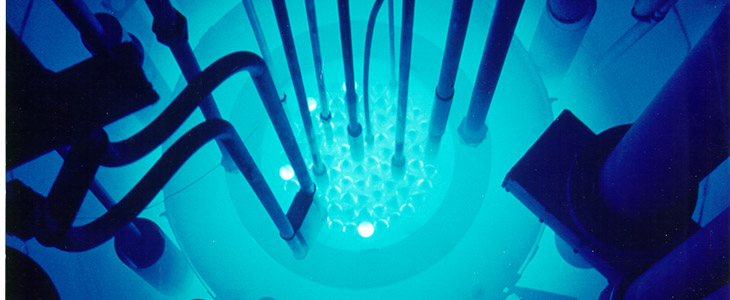
\includegraphics[width=0.9\textwidth]{01_introduction/pics/triga}
\caption{The TRIGA MARK II neutron reactor \cite{GeneralAtomics}.}
\label{fig:triga}
\end{figure}




\item[n-ToF] (neutron Time-of-Flight)~\cite{NTOF:00000} is a scientific collaboration with the aim of studying neutron-nucleus interactions. Over 30 institutes are active members of this collaboration, among them Atominstitut in Vienna. The n-ToF experiment is located at CERN where the experiments are carried out in a 200 m long experimental area. The knowledge stemming from the experimental results can then be applied in various fields ranging from nuclear technology and cancer therapy to astrophysics.

A pulsed beam of highly energetic protons (20~GeV/c) is produced by the Proton Synchrotron (PS) and aimed at a fixed lead spallation target. Each proton hitting the target produces around 300 neutrons of various energies. Initially highly energetic neutrons are slowed down by the target and by a slab of water placed behind it. This broadens their energy spectrum, which then ranges from meV (thermal neutrons) to GeV (fast neutrons). The neutrons are then sent through a 185~m long evacuated pipe to the experimental area, where they collide with another target or a sample. The radiation created by the collisions is detected by a set of dedicated detectors around the interaction point, as shown in figure~\ref{fig:ntof}. Having different energies, neutrons travel with different speeds, highly energetic ones reaching the target faster than those with low energies. The analysis of collisions with a precise timing allows for a determination of the interaction probability with the sample material as a function of energy of the incident neutrons.
\begin{figure}[!t]
\centering
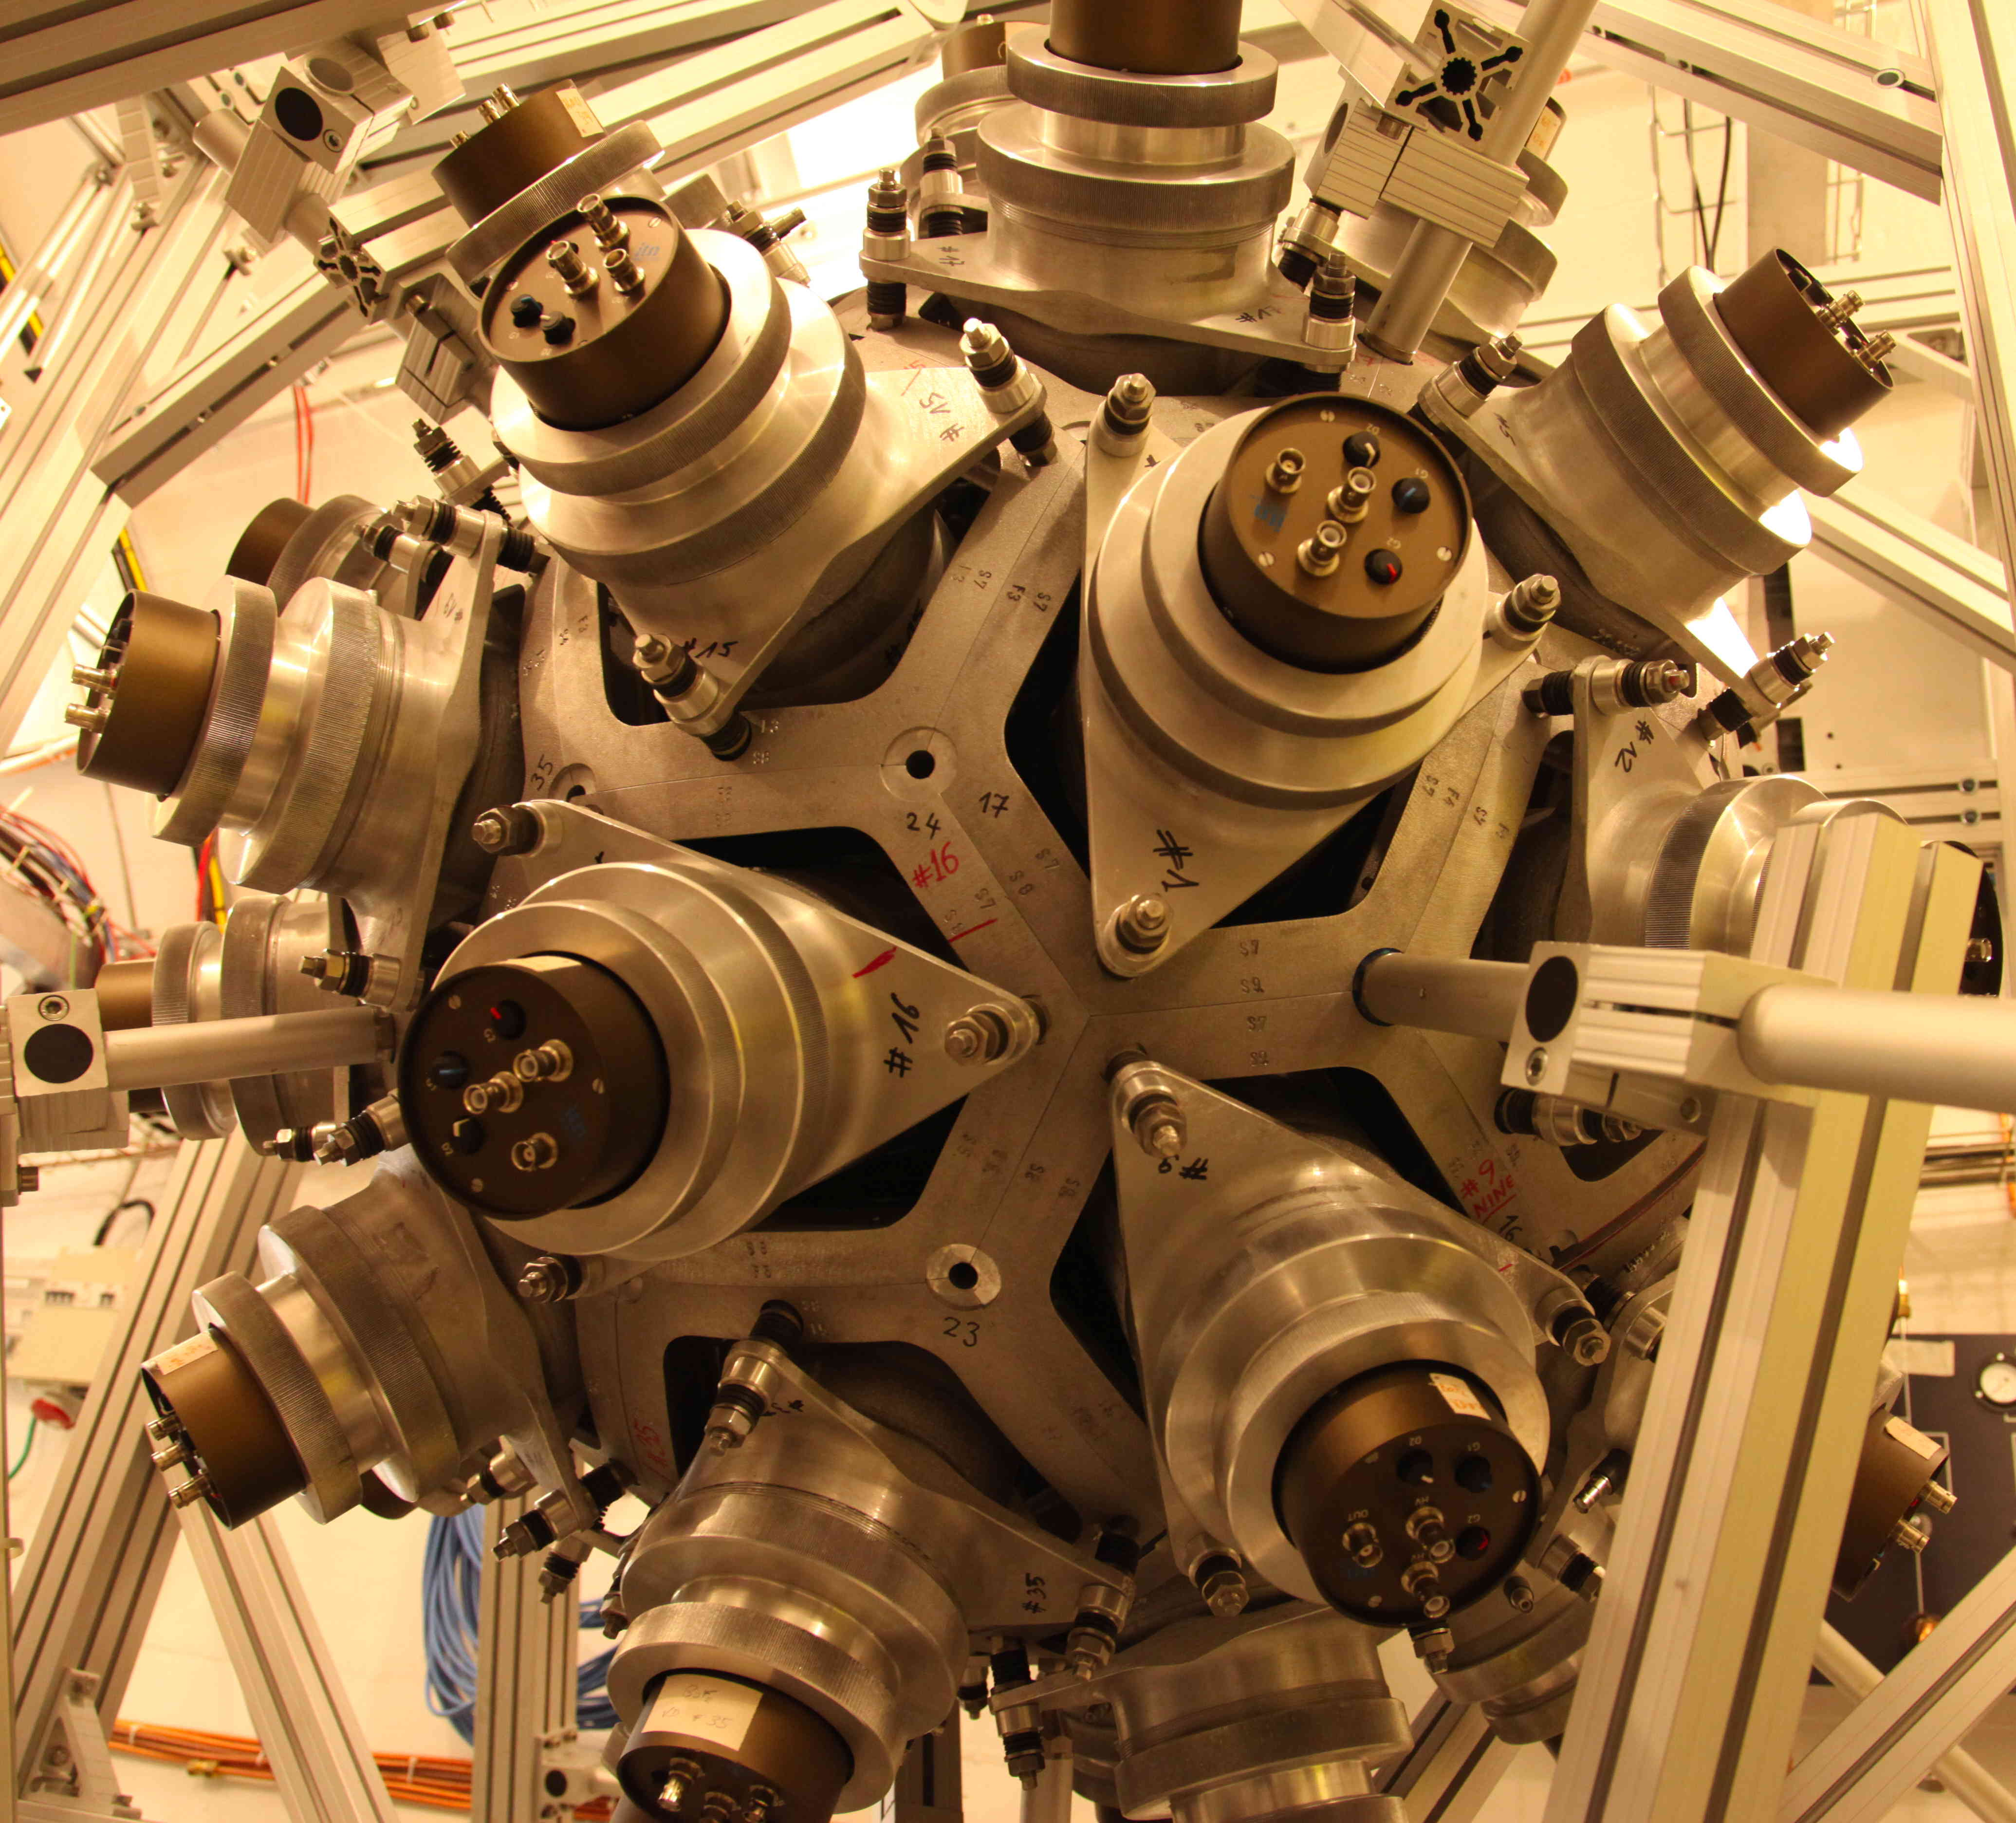
\includegraphics[width=0.9\textwidth]{01_introduction/pics/ntof}
\caption{The calorimeter in the n-ToF area \cite{Maximilien:1304589}.}
\label{fig:ntof}
\end{figure}
\end{description}





\section{The Large Hadron Collider}
\label{subsec:lhc}
A particle accelerator is a machine that accelerates beams of charged particles such as protons, electrons, ions etc. It generates electric fields that add kinetic energy to the particles, speeding them up. It then uses magnets to retain them within a defined trajectory and inside the evacuated beam pipe. The trajectory can be either linear (linear accelerators or LINACs) or circular (circular or cyclic accelerators). The former accelerate particles in a straight line, therefore the acceleration process only occurs once. The latter can accelerate particles many times while keeping them in orbit, but need a LINAC to pre-accelerate the particles before being injected in the loop.

Particle accelerators are used in numerous fields ranging from fundamental and material research, cancer treatment to industrial applications, such as biomedicine and material processing. Several types of accelerators exist: electrostatic accelerators, LINACs, cyclotrons, synchrocyclotrons, synchrotrons, synchrotron radiation sources and fixed-field alternating gradient accelerators (FFAGs).

The Large Hadron Collider (LHC, figure~\ref{fig:lhc}) at CERN is the largest particle collider in the world. It was build between 1998 and 2008 and was first successfully started in 2010 and operated until 2013 when it underwent a two-year long upgrade. Its second operational cycle started at the beginning of 2015.

The LHC is a 27~km long circular machine set up in a tunnel deep under the surface, ranging from 50 to 175~m below ground. It accelerates two proton beams to the energy of 6.5~TeV per beam before it makes them collide with each other with the energy of 13~TeV at four different interaction points around its circumference. 
\begin{figure}[!t]
\centering
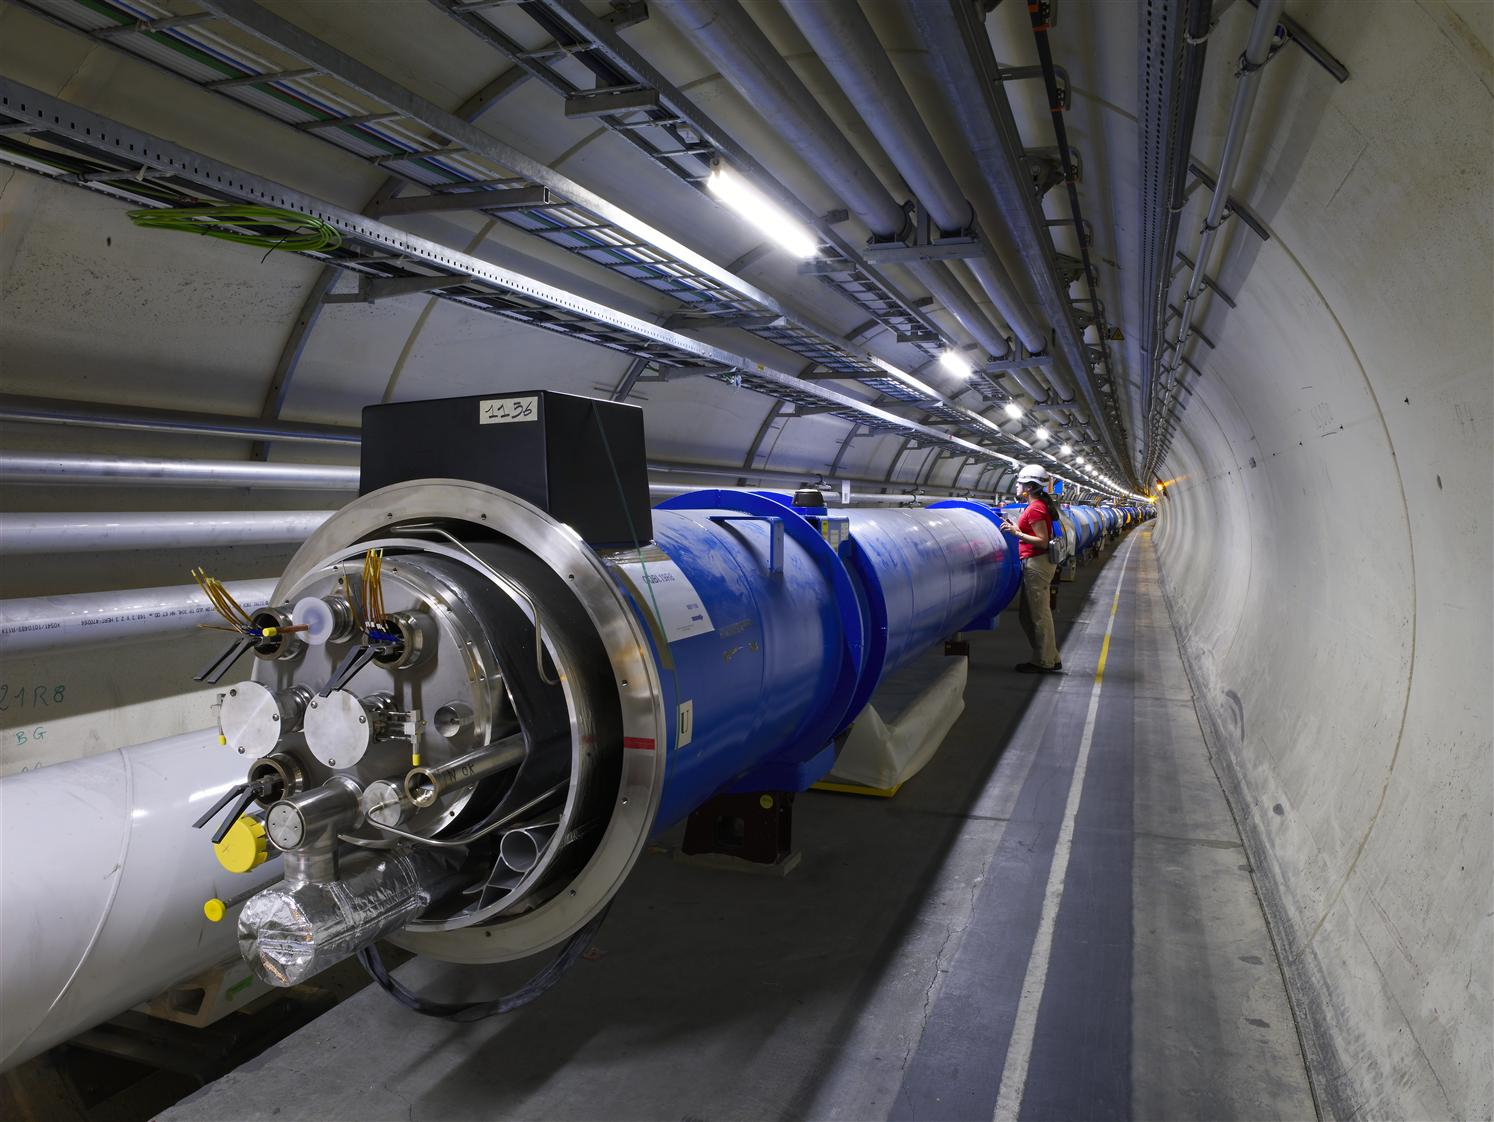
\includegraphics[width=0.9\textwidth]{01_introduction/pics/lhc}
\caption{The Large Hadron Collider \cite{Maximilien:1324852}.}
\label{fig:lhc}
\end{figure}
Hair-thin particle beams are guided inside two evacuated pipes with a $\sim$5~cm radius by means of magnetic field. Coils made up of a superconductive material are wound around the pipes in special patterns. When cooled down to -271 \textdegree C using liquid helium, they become superconductive; the resistivity of the material drops significantly, minimising the heat dissipation despite high electric currents. These produce strong magnetic fields which bend the particles and keep them in a circular trajectory. 

The protons travel bunched together in groups of $10^{11}$ per bunch. These bunches are accelerated when traversing the radio-frequency (RF) cavities with the frequency of the electromagnetic field equal to 400~MHz. This oscillating field creates 2.5~ns long buckets -- compartments for the bunches. Only one out of ten buckets is filled, so the bunches are spaced at 25~ns. This defines the machine's clock (40~MHz) as well as the maximum rate of collisions - the bunches travelling in the opposite direction cross at the intersections 40~million times per second. Around 20 collisions occur during every bunch crossing, yielding the maximum collision rate of the order of $10^9$~s$^{-1}$. The number of collisions will increase in the following years; the number of particles per bunch will be increased and the transverse spread of the bunches will be decreased. The bunch density will therefore be increased, which will in turn increase the collision probability -- the cross-section. The original design number of collisions accumulated over the years of operation is presented in the form of integrated luminosity~\cite{} and is of the order of 300~fb$^{-1}$ (inverse femtobarn). After the planned upgrades in 2020, the High-Luminosity LHC~\cite{} will achieve up to 3000~fb$^{-1}$.

\section{The ATLAS experiment}
ATLAS (short for A Toroidal Lhc ApparatuS, figure~\ref{fig:atlas})~\cite{} is a particle physics experiment at CERN. Its purpose is to verify current theories and to search for new discoveries by observing and analysing high energy proton-proton collisions produced by the LHC. It is the biggest experiment at CERN by dimensions (45~m in length and 26~m in height) and the number of people involved (more than 3000 physicists and engineers).
\begin{figure}[!t]
\centering
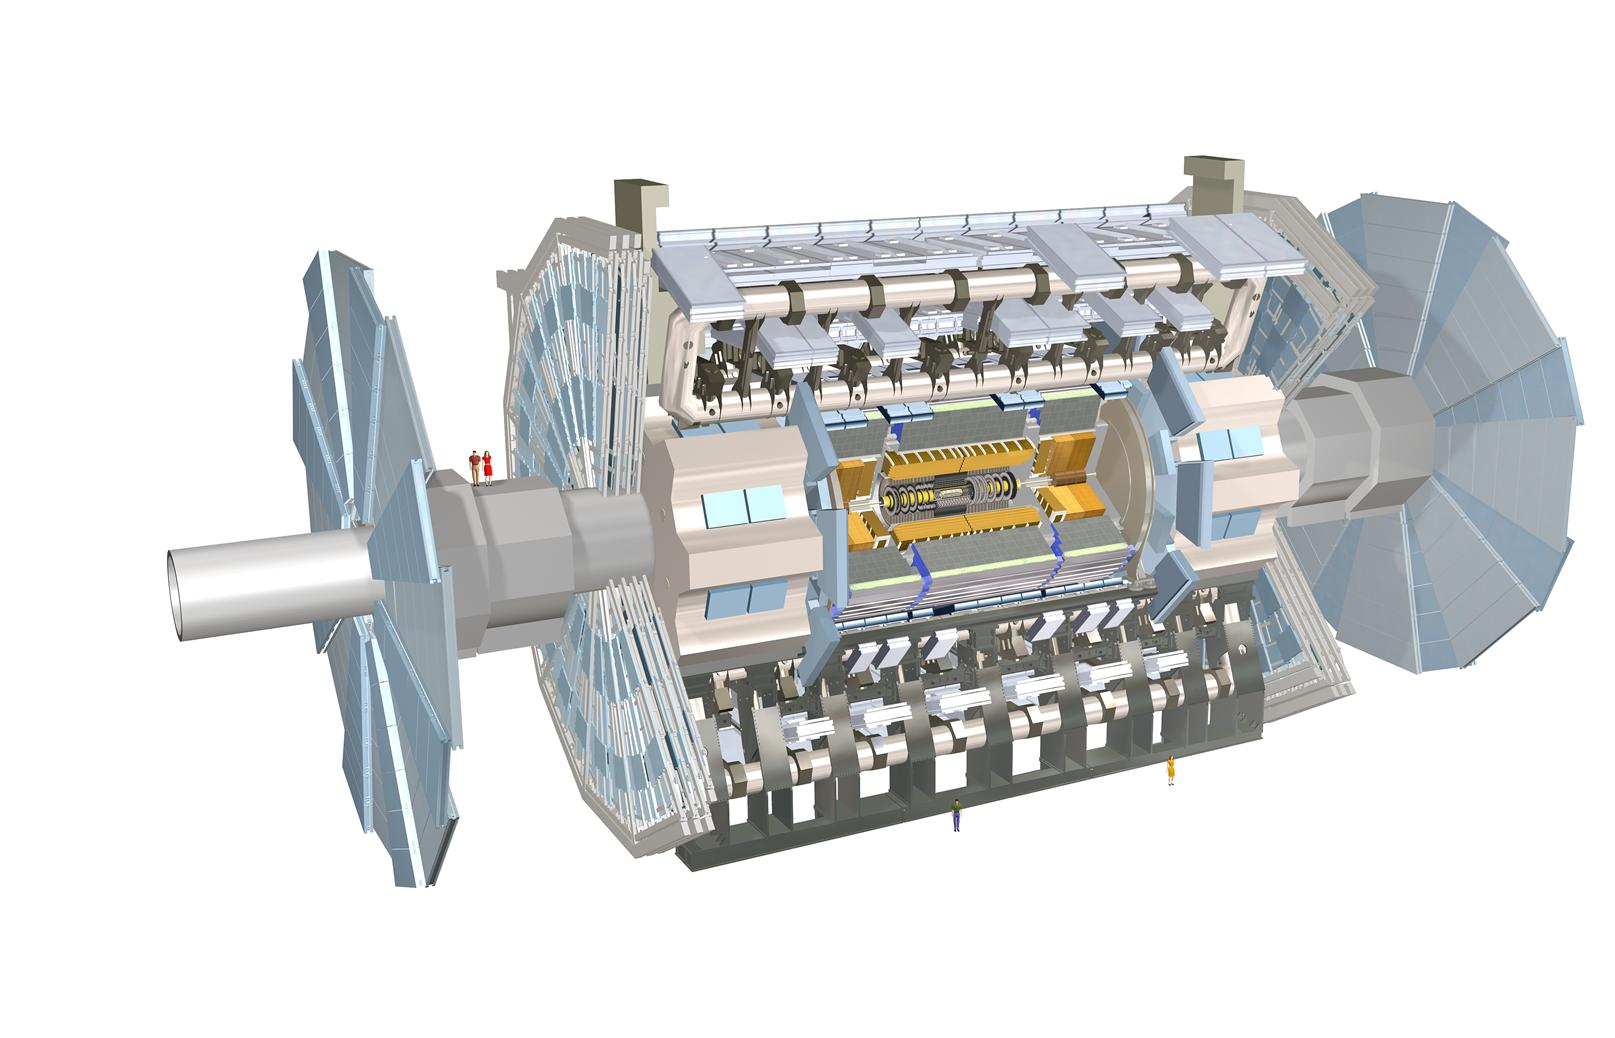
\includegraphics[width=0.9\textwidth]{01_introduction/pics/atlas3}
\caption{The ATLAS Experiment \cite{Pequenao:1095924}.}
\label{fig:atlas}
\end{figure}
The ATLAS experiment consists of a number of detectors, each designed to measure a specific property of the particles and photons produced during the collision. The closest to the collision point is the Inner Detector (ID), which consists of scintillating elements, a Transition Radiation Tracker and of the several layers of highly spatially segmented semiconductor sensors, which record single points of the incident particles. These points are later reconstructed into particle tracks. In addition, a strong magnetic field of 2~T curves the paths of the charged particles, which in turn allows the ID to identify an individual particle's charge and momentum. The next two parts are the electromagnetic and tile calorimeter. These detectors weigh a few thousand tonnes and measure the energy that the particles deposit in the material. The only particles that make it through the calorimeters are neutrinos and muons. The former cannot be detected with the detectors in ATLAS. The latter however are detected by the Muon Spectrometer, a set of large detector plates placed all around the calorimeters. The last is the superconductive magnet which provides the magnetic field to allow the Muon Spectrometer to measure muon momenta. The ID has its own set of magnets that are used for the same purpose. To sum up, the Inner Detector measures the charge and momenta of the particles, the calorimeters measure their energies, the Muon Spectrometer measures muon tracks and momenta and the magnets provide magnetic fields, which curve the trajectories of the charged particles, allowing for identification of particle momenta.

The ATLAS detector has been designed to measure every collision taking place in its core. With 25~ns between collisions, this makes up 40~million collisions per second. The maximum realistic achievable rate of recording is approximately 100~kHz~\cite{}. A recorded collision is referred to as an event. Every event holds information acquired by all the detectors within ATLAS. This amounts to approximately $\sim$$10^6$ channels of data, yielding an event size of approximately 10~MB. Therefore the data rate at the maximum achievable rate is 3~TB/s. To reduce the amount of data stored a special classification system with a complex trigger logic, which is in place to decide which events should be stored and analysed further. It reaches a decision in the order of tens of microseconds after an event. If this is the case, the data acquisition system triggers the readout of the entire detector. This way the recorded event rate is reduced from 100~kHz to $\sim$500~Hz.

A complex Trigger and Data Acquisition system (TDAQ) is in place to distribute the clock signal, configure the detectors, perform data acquisition and handle the output data. The data are then stored at the CERN computer centre and distributed across the globe by means of the GRID -- a distributed data analysis and data storage system.



% ---------------------------------------------------------------------------------------------------------------
\section{Particle detectors}
Particle detectors, or radiation detectors, have first come into use at the end of the 19th century. At that time Wilhelm R\"ontgen used a photographic plate onto which he shone X-rays. Soon after, in 1912, Victor F. Hess discovered cosmic rays during a balloon flight. This paved the way for development of particle detectors. A cloud chamber was designed -- a chamber filled with a supersaturated vapour of water or alcohol. If a highly energetic particle traversed the chamber, the mixture ionised, creating condensation nuclei. These traces were visible and were photographed. The particle detectors developed later relied on different types of interaction between the incident particles and the detector material, e.g. transition radiation, Cherenkov radiation and ionisation. The bubble chamber invented in 1952 used a superheated transparent liquid -- a liquid heated just below its boiling point. A particle ionised the liquid, forming microscopic bubbles along its trajectory. Then followed the spark chamber and the wire chamber where the particle ionised the gas, causing a spark between two parallel plates at a high potential difference. These are nowadays used in a handful of experiments and may often be seen in museums as showcases. Next were ionisation chambers, which measured the induced current of the free ionised charges moving in an externally applied electric field. Finally in the 1960s, semiconductor detectors were introduced. Their principle of operation is similar to that of an ionisation chamber, with the difference that a semi-conductive material is used as an ionisation medium instead of gas. Nowadays an ensemble of several types of detectors is used as a specialised detector system. Many considerations need to be taken into account when designing such a system: detector geometry, segmentation, event rate, efficiency, readout, support structures, cabling, cooling, cost etc.

Particle detectors can be divided in two groups: tracking detectors and calorimeters. The former are designed to measure  particle momentum, charge, origin and direction of flight, with a minimal impact on their flight path or energy with the aim to optimise the spatial resolution. The calorimeters, on the other hand, measure the energy of the particles by stopping them. This means they need to be heavy and dense. A typical physics experiment nowadays consists of a tracking detector enclosed by a calorimeter. This way the energy, charge and momentum can be derived for every particle created in the collision.

%History and use (1 pg)
%Comparison table (2 pg)

%\subsection{Semiconductor sensors}



